\documentclass{exam}

\usepackage{units} 
\usepackage{graphicx}
\usepackage[fleqn]{amsmath}
\usepackage{cancel}
\usepackage{float}
\usepackage{mdwlist}
\usepackage{booktabs}
\usepackage{cancel}
\usepackage{polynom}
\usepackage{caption}
\usepackage{fullpage}
\usepackage{xfrac}
\usepackage{enumerate}

\newcommand{\dg}{\ensuremath{^\circ}} 
\everymath{\displaystyle}

\printanswers

\title{Math 142 Notes \\ Section 7.1}

\date{\today}

\begin{document}

  \maketitle
  \tableofcontents

  \section{Identities}
  \subsection{Pythagorean Identities}
  \begin{align*}
    \sin^2 x + \cos^2 x & = 1 \\
    \tan^2 x + 1        & = \sec^2 x \\
    \cot^2 x + 1        & = \csc^2 x \\
  \end{align*}

  \subsection{Even/Odd Identities}
  \begin{align*}
    \sin(-x) & = - \sin x \\
    \cos(-x) & = \cos x \\
    \tan(-x) & = - \tan x \\
  \end{align*}

  Show with:
  \begin{itemize*}
    \item unit circle
    \item y-axis (cosine) or origin (sine and tangent) symmetry in graph
  \end{itemize*}

  \subsection{Cofunction Identities}
  \begin{align*}
    \sin \left( \frac{\pi}{2} - u \right) &= \cos u \\
    \cos \left( \frac{\pi}{2} - u \right) &= \sin u \\
    \tan \left( \frac{\pi}{2} - u \right) &= \cot u \\
    \\
    \sec \left( \frac{\pi}{2} - u \right) &= \csc u \\
    \csc \left( \frac{\pi}{2} - u \right) &= \sec u \\
    \cot \left( \frac{\pi}{2} - u \right) &= \tan u \\
  \end{align*}

  Show with right triangle.

  Show with graph reflection:

  \begin{figure}[H]
    \centering
    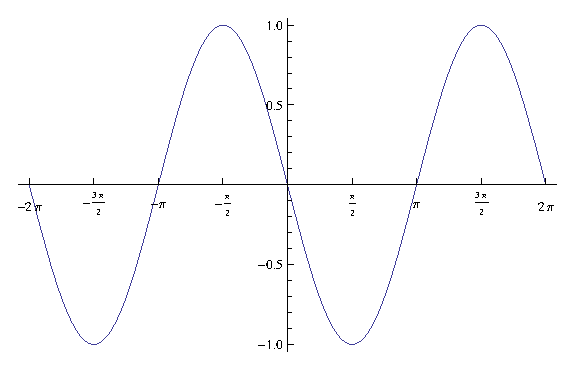
\includegraphics[scale=0.7]{sine_negative_x}
    \caption{$g(x) = \sin(-x)$}
  \end{figure}

  \begin{figure}[H]
    \centering
    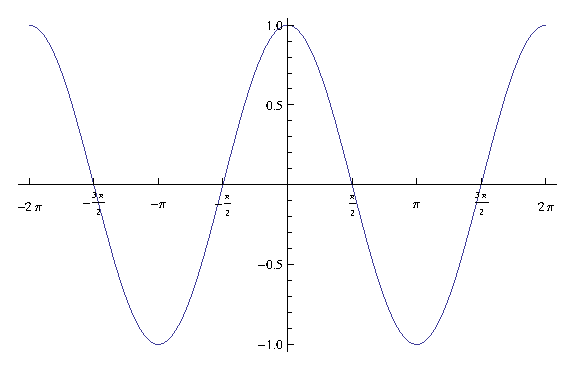
\includegraphics[scale=0.7]{cosine_x}
    \caption{$g(x - \sfrac{\pi}{2}) = \sin(- ( x - \sfrac{\pi}{2}))$}
  \end{figure}

  \begin{figure}[H]
    \centering
    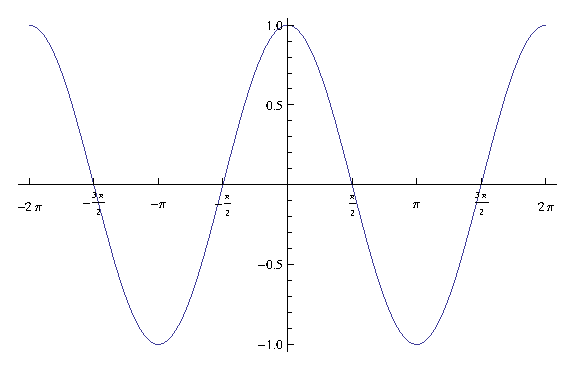
\includegraphics[scale=0.7]{cosine_x}
    \caption{$g(x) = \cos(-x)$}
  \end{figure}

  \begin{figure}[H]
    \centering
    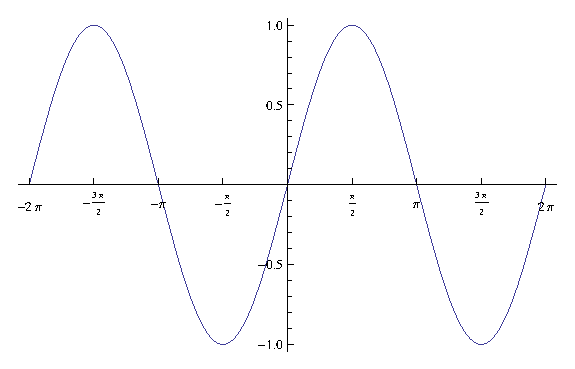
\includegraphics[scale=0.7]{sine_x}
    \caption{$g(x - \sfrac{\pi}{2}) = \cos(- ( x - \sfrac{\pi}{2}))$}
  \end{figure}

  \section{Proving Identities}

  \begin{itemize*}
    \item start with more complicated side
    \item use identities and algebra to simplify
    \item when in doubt, convert everything to sine/cosine
    \item multiplying $(a + b)$ by $(a - b)$ to get $a^2 - b^2$ is sometimes useful
  \end{itemize*}

  Do examples from book.

  \section{Trigonometric substitution}
  See exercises 89-94.  


\end{document}
